% ============================================================================
% ClaimSense at IndicClaimVer@FIRE 2026 -- System Description Paper
% ============================================================================
% This file targets the official CEUR-WS "ceurart" LaTeX class
% (https://www.overleaf.com/latex/templates/template-for-submissions-to-
%  ceur-workshop-proceedings-ceur-ws-dot-org/hpvjjzhjxzjk).
%
% HOW TO USE:
%   1. Open the official CEUR-WS Overleaf template project (link above) --
%      it already bundles ceurart.cls and its dependencies. Do NOT try to
%      compile this file standalone without that class file present.
%   2. Replace/add this file as the project's main .tex file.
%   3. Add references.bib (companion file, same folder) to the project.
%   4. Add the two Neo4j screenshots (see the two \KGFIGUREPLACEHOLDER
%      blocks below) as image files and swap in the commented-out
%      \includegraphics lines once you have them.
%   5. Fill in every [PLACEHOLDER] marked below (affiliation, emails,
%      conference metadata, ORCIDs) before submission.
%
% ENCODING NOTE: this file is pure ASCII/Latin-script by design, so it
% compiles cleanly under plain pdflatex (as the official CEUR toolchain
% expects) with no extra font/engine setup. A few short example words
% that exist in Bengali/Devanagari script in the plain-English draft
% (system_description_paper.md) are given here in italicized
% transliteration instead of literal script glyphs (e.g. *Bamangachi*
% rather than the Bengali spelling) for this reason. If you specifically
% want literal Indic-script examples typeset in the PDF, switch to
% XeLaTeX or LuaLaTeX and add \usepackage{fontspec} plus an installed
% Bengali/Devanagari font via \newfontfamily -- verify ceurart still
% compiles under that engine before relying on it, and note that CEUR-WS
% output is generally expected to be produced with plain pdflatex.
% ============================================================================

\documentclass[
%twocolumn,
%hf,
]{ceurart}

\usepackage{booktabs}
\usepackage{tikz}
\usetikzlibrary{positioning, arrows.meta, shapes.geometric, fit}

\sloppy

\begin{document}

%--- Front matter -------------------------------------------------------

\copyrightyear{2026}
\copyrightclause{Copyright for this paper by its authors.
  Use permitted under Creative Commons License Attribution 4.0
  International (CC BY 4.0).}

\conference{FIRE 2026: Forum for Information Retrieval Evaluation,
  IndicClaimVer Shared Task, [Month placeholder] 2026, [City, Country placeholder]}

\title{ClaimSense at IndicClaimVer@FIRE 2026: Retrieval-Augmented and
  Knowledge-Graph-Boosted Multilingual Claim Verification}

% One \author line per team member. Fill in email/orcid/url as needed;
% remove the [...] block entirely for an author with no such metadata.
\author[1]{Sayan De}[%
  email=[email placeholder]
]
\author[1]{Koushiki Chakraborty}[%
  email=[email placeholder]
]
\author[1]{Nirnit Roy}[%
  email=[email placeholder]
]
\author[1]{Anindita Dutta}[%
  email=[email placeholder]
]
\author[1]{Archismita Das}[%
  email=[email placeholder]
]

\address[1]{[Affiliation / institution name placeholder]}

%--- Abstract + keywords -------------------------------------------------

\begin{abstract}
We present the ClaimSense system submitted to the IndicClaimVer@FIRE 2026
shared task, which targets multilingual (English, Hindi, Bengali, and
code-mixed) claim verification over the IndicClaimBuster dataset. We
participated in both subtasks. For \textbf{Subtask 1} (closed-domain
evidence retrieval and veracity prediction over a fixed evidence pool),
our system combines a per-language BM25 baseline, dense multilingual
retrieval using \texttt{intfloat/multilingual-e5-base}, and a Neo4j
knowledge-graph-boosted reranking stage that reranks the dense top-10
candidates by inverse-document-frequency-weighted entity overlap,
computed through a multi-stage Wikidata entity-linking cascade (exact
match, code-mixed retry, Bengali morphological normalization, fuzzy
search, semantic reranking, and an LLM fallback for the hardest cases).
Veracity is predicted either by GPT-4o-mini reasoning over the top-1
retrieved evidence, or by a standalone MuRIL-based binary classifier
fine-tuned with hyperparameters found via Optuna search. For
\textbf{Subtask 2} (open-domain web-based verification), our system
generates native-language and English search queries deterministically,
retrieves evidence via the Tavily web search API, ranks it through a
pipeline of BM25, multilingual sentence-embedding similarity, and a
persistent Neo4j entity graph (optionally enriched with cross-lingual
Wikidata QID linking), fuses the three rankings with Reciprocal Rank
Fusion, fetches full article text for the top-3 fused results, and
produces a grounded veracity verdict and justification using a large
language model under a strict no-hallucination prompting regime. On the
official test set, our submitted Subtask 1 system reaches a veracity
macro-F1 of 78.05 (English), 85.88 (Hindi), 82.46 (Bengali), and 79.94
(code-mixed); our Subtask 2 system reaches a veracity macro-F1 of 76.91
(English), 68.97 (Hindi), 62.92 (Bengali), and 36.51 (code-mixed). On our
own development-set ablations, knowledge-graph-boosted retrieval is the
strongest Subtask 1 retrieval configuration we tested (Success@3 =
0.8395, nDCG@3 = 0.5748 on the combined train+dev set, beating a
dense-retrieval-only baseline at every entity-overlap weight tested in
$[0.01, 0.05]$), and LLM-based verification is the strongest Subtask 2
configuration we tested (macro-F1 = 0.8039 on the 631-claim development
set), outperforming a reused standalone MuRIL classifier (macro-F1 =
0.6820) on the same claims. We discuss language-specific weaknesses --
Bengali and, most severely, code-mixed text are consistently the
hardest buckets across every retrieval and verification method we
tried, in both our own ablations and the official test-set results --
along with our ranking-fusion design decisions and directions for
future work.
\end{abstract}

\begin{keywords}
  Claim Verification \sep
  Multilingual Natural Language Processing \sep
  Knowledge Graphs \sep
  Information Retrieval \sep
  Large Language Models \sep
  Entity Linking \sep
  Reciprocal Rank Fusion \sep
  FIRE 2026 \sep
  IndicClaimVer
\end{keywords}

\maketitle

% ============================================================================
\section{Introduction}
% ============================================================================

Automated fact verification for low-resource and code-mixed Indic
languages faces two compounding difficulties: (i) claims and evidence are
often expressed in a mix of scripts and registers -- formal news prose,
informal social-media phrasing, and code-mixed Hindi--Bengali--English
sentences -- and (ii) the evidence a verification system must reason over
may either come from a small, fixed pool (a \emph{closed} retrieval
setting) or from the open web (an \emph{open-domain} setting), each of
which demands a different system design. The IndicClaimVer@FIRE 2026
shared task, built on the IndicClaimBuster dataset
\cite{pal-etal-2025-indicclaimbuster}, evaluates both settings directly
through two subtasks:

\begin{itemize}
  \item \textbf{Subtask 1} (closed evidence retrieval + veracity
    prediction): given a claim and a fixed pool of roughly 13{,}000
    evidence passages, retrieve the top-3 most relevant passages and
    predict whether the claim is \texttt{SUPPORTS}ed or
    \texttt{REFUTES}d.
  \item \textbf{Subtask 2} (open-domain retrieval + veracity
    prediction): given a claim only, retrieve supporting or refuting
    evidence from the live web, and produce a veracity verdict together
    with a natural-language justification grounded in that evidence.
\end{itemize}

Our team, ClaimSense, built independent but architecturally related
pipelines for the two subtasks. Both pipelines share a design
philosophy: combine a fast lexical signal (BM25), a semantic signal
(multilingual sentence embeddings), and a symbolic, inspectable signal
(a Neo4j knowledge graph built from extracted entities), rather than
relying on a single neural reranker. We found this combination gives
both stronger retrieval quality and a more debuggable system -- every
ranking decision can be traced back to an explicit score component (a
BM25 score, a cosine similarity, or an entity-overlap count visible
directly in the graph).

This paper documents both systems in full: data handling, retrieval
architecture, knowledge-graph construction and entity linking, veracity
prediction (both an LLM-based path and a standalone fine-tuned
classifier), the ablations that shaped our final configuration, and the
official and development-set results for both subtasks.

\paragraph{Contributions.}
\begin{enumerate}
  \item An entity-overlap knowledge-graph reranking stage for
    closed-domain retrieval that we show, through a controlled weight
    sweep, robustly improves over dense-retrieval-only ranking on both
    Success@3 and nDCG@3 across a wide range of its single
    hyperparameter.
  \item A multi-stage, cost-aware entity-linking cascade for
    Indic-script text that combines free Wikidata lookups (exact match,
    code-mixed retry, Bengali morphological stripping, fuzzy search)
    with a last-resort, disk-cached LLM fallback used only when the
    free cascade is structurally weak or unconfident.
  \item A deterministic (LLM-free) bilingual query-generation stage for
    open-domain retrieval that preserves exact numeric tokens (case
    counts, percentages, dates) shown empirically to matter for pinning
    retrieval to the correct day's article.
  \item A Reciprocal-Rank-Fusion-based evidence ranker that combines
    lexical, semantic, and knowledge-graph signals without needing to
    calibrate their raw score scales against one another.
  \item A grounded LLM verification prompt with explicit anti-hedging
    and anti-hallucination constraints, checked both by instruction and
    by post-hoc validation of the model's output.
  \item A reuse analysis showing that the same fine-tuned MuRIL
    classifier, applied without modification to both subtasks, is
    consistently and substantially outperformed by LLM-based veracity
    prediction on both -- a result we report honestly, including a
    methodological correction we made to our own development-set
    evaluation (Section~\ref{sec:results-st2}) after discovering an
    earlier scoring inconsistency.
\end{enumerate}

% ============================================================================
\section{Related Work}
% ============================================================================

Our system builds directly on the IndicClaimBuster resource
\cite{pal-etal-2025-indicclaimbuster}, which introduced the multilingual
claim--evidence--label dataset underlying both subtasks of this shared
task.

Our retrieval design follows the now-standard ``lexical + dense +
fusion'' pattern used across recent multilingual information retrieval
systems: a probabilistic bag-of-words ranker (BM25, the Okapi
formulation \cite{robertson2009probabilistic}) provides a strong,
script-agnostic lexical baseline; a multilingual dense bi-encoder
(\texttt{intfloat/multilingual-e5-base} \cite{wang2024multilingual})
provides a semantic signal robust to vocabulary mismatch across
languages; and, for Subtask 2, Reciprocal Rank Fusion
\cite{cormack2009reciprocal} combines multiple rank-based signals
without requiring cross-signal score calibration. Our knowledge-graph
reranking stage is inspired by entity-centric relevance signals used in
knowledge-graph-augmented retrieval and fact-verification systems, but
we deliberately keep the graph schema minimal (claim/evidence/entity
nodes and mention/overlap edges) rather than modeling a full knowledge
base, since our goal is a transparent ranking booster, not a
general-purpose knowledge base built on Wikidata
\cite{vrandecic2014wikidata} and served through Neo4j \cite{neo4j}. For
entity linking, we build a cost-aware cascade over Wikidata's public
SPARQL and \texttt{wbsearchentities} endpoints, escalating to a large
language model only for the hardest, highest-value cases -- a design
choice made explicit and measured in
Section~\ref{sec:st1-entity-linking}.

For veracity prediction, we use two complementary approaches also common
in the fact-verification literature: (i) prompting a general-purpose
instruction-following LLM (GPT-4o-mini \cite{openai2024gpt4omini} for
Subtask 1, and for Subtask 2, a model from the Gemini family
\cite{geminiteam2023gemini} -- see the backend note in
Section~\ref{sec:st2-verification}) with a strict, evidence-grounded
decision rule, and (ii) fine-tuning a smaller, dedicated multilingual
encoder (MuRIL \cite{khanuja2021muril}) as a lower-cost,
offline-capable classifier, following a fine-tuning and hyperparameter
search recipe built on Optuna \cite{optuna}. We compare both directly
against each other on both subtasks.

% ============================================================================
\section{Task Description}
% ============================================================================

\subsection{Subtask 1 -- Closed Evidence Retrieval and Veracity Prediction}

Given a claim \texttt{\{ID, Text\}} and a fixed pool of evidence
passages \texttt{\{ID, Evidence\}} (approximately 13{,}333 items for the
development/training split, 28{,}618 for the official test split), the
system must return, for each claim, the three evidence passages ranked
most-to-least relevant, plus a single veracity label, \texttt{SUPPORTS}
or \texttt{REFUTES}. Systems are scored on retrieval quality --
Success@3 and nDCG@3 against the single gold evidence item per claim --
and on veracity accuracy/macro-F1 against the gold label. This is a
\emph{closed} setting: no live web access is permitted or needed; every
claim's supporting or refuting evidence is guaranteed to exist somewhere
in the fixed pool.

\subsection{Subtask 2 -- Open-Domain Retrieval and Veracity Prediction}

Given a claim only (no fixed evidence pool), the system must retrieve
its own supporting or refuting evidence from the open web, and produce
a structured verdict record \texttt{\{ID, Evidence, Prediction,
Justification\}}, where \texttt{Evidence} is a concise,
evidence-grounded summary, \texttt{Prediction} is exactly
\texttt{SUPPORTS} or \texttt{REFUTES}, and \texttt{Justification}
explains the verdict with explicit reference to the retrieved evidence.
Unlike Subtask 1, there is no fixed pool and no guarantee that any
single passage directly confirms or denies the claim -- the system must
locate, rank, and reason over live web content itself.

\subsection{Languages}

Both subtasks cover four language conditions: English, Hindi, Bengali,
and \textbf{code-mixed} text (informal claims that mix Latin and Indic
scripts within a single sentence, common in social-media-sourced
misinformation). Code-mixed and Bengali text are, across both of our
subtasks and every retrieval method we tested, the consistently hardest
buckets -- a pattern we discuss in Section~\ref{sec:discussion}.

% ============================================================================
\section{Datasets}
% ============================================================================

\subsection{Subtask 1}

\begin{table}[h]
  \centering
  \caption{Subtask 1 dataset statistics.}
  \label{tab:st1-data}
  \begin{tabular}{@{}lrrl@{}}
    \toprule
    Split & Claims & Evidence pool size & Notes \\
    \midrule
    Train & 4{,}536 & 13{,}333 (shared) & 3{,}040 \texttt{SUPPORTS} / 1{,}496 \texttt{REFUTES} \\
    Dev & 1{,}134 & 13{,}333 (shared) & Used for all ablations in Section~\ref{sec:results-st1} \\
    Official test & 3{,}900 & 28{,}618 & 1{,}200 EN + 1{,}200 HI + 1{,}200 BN + 300 CodeMix \\
    \bottomrule
  \end{tabular}
\end{table}

\subsection{Subtask 2}

\begin{table}[h]
  \centering
  \caption{Subtask 2 dataset statistics.}
  \label{tab:st2-data}
  \begin{tabular}{@{}lrl@{}}
    \toprule
    Split & Claims & Notes \\
    \midrule
    Dev & 631 & Gold \texttt{Label} provided; used for our development metrics \\
    Official test & 1{,}009 & 299 EN + 278 HI + 258 BN + 174 CodeMix \\
    \bottomrule
  \end{tabular}
\end{table}

For both subtasks, claim language is either provided directly by the
source file (Subtask 2's four per-language test files, and our own
filename-based tagging convention) or detected via a lightweight,
character-count-weighted script classifier for Subtask 1 (Devanagari
and Bengali Unicode ranges are weighted $2\times$ relative to Latin
characters, since a single Latin word inside an otherwise-Devanagari
sentence should not flip the detected language). We additionally flag a
claim as \textbf{code-mixed} whenever it contains both an Indic-script
run and a Latin-script run of at least four characters.

% ============================================================================
\section{System Architecture -- Subtask 1}
\label{sec:st1-arch}
% ============================================================================

\subsection{Pipeline Overview}

Figure~\ref{fig:st1-pipeline} shows the full Subtask 1 pipeline. The
production configuration is \textbf{Dense retrieval (top-10)
$\rightarrow$ Knowledge-Graph-boosted rerank (top-3) $\rightarrow$
Veracity prediction}. BM25 is retained as a per-language lexical
baseline used to validate that dense retrieval is actually the stronger
signal before committing to it (Section~\ref{sec:results-st1}), but it
is not part of the final scored chain.

\begin{figure}[h]
  \centering
  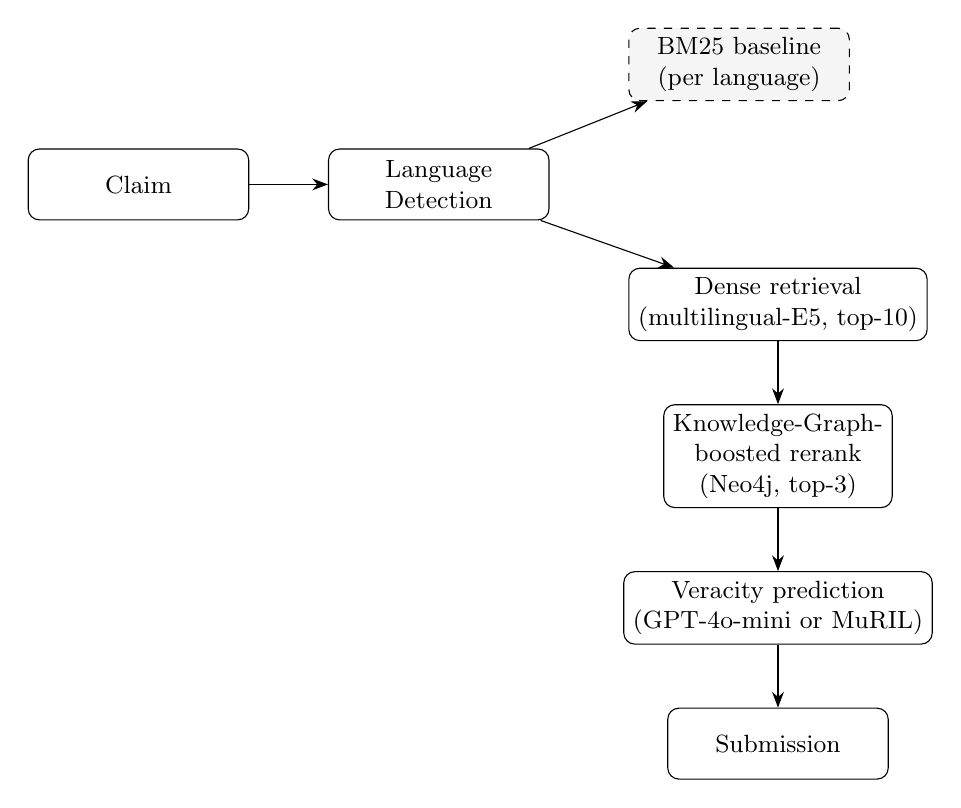
\begin{tikzpicture}[
      node distance=8mm and 10mm,
      box/.style={draw, rounded corners, align=center, minimum height=9mm, minimum width=28mm, font=\small},
      baseline/.style={box, dashed, fill=gray!8},
      arr/.style={-{Stealth[length=2mm]}}
    ]
    \node[box] (claim) {Claim};
    \node[box, right=of claim] (lang) {Language\\Detection};
    \node[baseline, above right=6mm and 10mm of lang] (bm25) {BM25 baseline\\(per language)};
    \node[box, below right=6mm and 10mm of lang] (dense) {Dense retrieval\\(multilingual-E5, top-10)};
    \node[box, below=of dense] (kg) {Knowledge-Graph-\\boosted rerank\\(Neo4j, top-3)};
    \node[box, below=of kg] (ver) {Veracity prediction\\(GPT-4o-mini or MuRIL)};
    \node[box, below=of ver] (sub) {Submission};

    \draw[arr] (claim) -- (lang);
    \draw[arr] (lang) -- (bm25);
    \draw[arr] (lang) -- (dense);
    \draw[arr] (dense) -- (kg);
    \draw[arr] (kg) -- (ver);
    \draw[arr] (ver) -- (sub);
  \end{tikzpicture}
  \caption{Subtask 1 pipeline. BM25 (dashed) is a validation baseline,
    not part of the final scored chain.}
  \label{fig:st1-pipeline}
\end{figure}

\subsection{Dense Retrieval}

We encode every claim and every evidence passage with
\texttt{intfloat/multilingual-e5-base} (768-dimensional embeddings),
using the E5 family's documented asymmetric \texttt{"query: "} /
\texttt{"passage: "} text prefixing \cite{wang2024multilingual}. We
selected E5 over an earlier multilingual sentence-embedding model
(\texttt{paraphrase-multilingual-mpnet-base-v2}) specifically because
that earlier model's own published training-language coverage does not
include Bengali, which produced catastrophic Bengali dense-retrieval
Success@3 (0.207) in an early validation gate; E5 is trained on mC4,
which covers Bengali, and is purpose-built for asymmetric query/passage
retrieval rather than paraphrase similarity. Embeddings are cached to
disk (hashed by text content, namespaced by model name) so re-encoding
is never repeated across pipeline runs. We evaluated two
dense-retrieval variants -- a full-pool cosine search and a
language-partitioned search restricted to same-language evidence -- and
found them statistically indistinguishable
(Section~\ref{sec:results-st1}); we report the full-pool variant as our
primary dense baseline.

\subsection{Knowledge-Graph-Boosted Reranking}
\label{sec:st1-kg}

We build a Neo4j graph with \texttt{Claim}, \texttt{Evidence}, and
\texttt{Entity} node types, connected by \texttt{MENTIONS} edges (from a
claim or evidence passage to each entity it mentions) and
\texttt{HAS\_MENTION} $\rightarrow$ \texttt{LINKS\_TO} edges recording
the specific surface-form mention and its resolved Wikidata entity.
Given a claim's dense top-10 candidates, we rerank them by a single
Cypher query that computes each candidate's entity overlap with the
claim, \textbf{weighted by inverse document frequency}: a shared entity
that appears in only a few documents across the whole corpus contributes
close to a full point of overlap score, while a shared entity that
appears in thousands of documents (e.g., a country or a national
political figure) contributes close to zero. This IDF weighting was
itself an empirical fix: an earlier flat-count overlap scheme (every
shared entity counted equally) \emph{underperformed} plain dense
retrieval (Success@3 0.7834 vs.\ 0.8312 on the full train+dev set),
because common entities dominated the score without carrying real
disambiguating value. After switching to IDF weighting, we swept the
single scaling hyperparameter (\texttt{ENTITY\_OVERLAP\_WEIGHT}) over
the range $[0.0, 2.0]$ on the full 5{,}670-claim train+dev set and found
a robust improving region: \textbf{every weight in $[0.01, 0.05]$ beat
dense-retrieval-only on both Success@3 and nDCG@3}, with a maximum at
weight $= 0.02$ (Section~\ref{sec:results-st1}, Table~\ref{tab:sweep}).

We additionally investigated a cluster-density penalty (DBSCAN-based
disambiguation \cite{ester1996dbscan}, penalizing candidates that fall
inside a dense, low-specificity evidence cluster while sharing zero
entity overlap with the claim). This was found to make retrieval
\textbf{strictly worse at every nonzero penalty weight tested} -- at
production scale, DBSCAN with the tuned similarity threshold collapsed
into a single giant cluster per language rather than isolating
genuinely confusable sub-events, turning the penalty into an
indiscriminate demotion rather than a targeted disambiguation signal.
This component is implemented but disabled in the final system; we
report the full experiment in Section~\ref{sec:results-st1} for
completeness.

\begin{figure}[h]
  \centering
  \includegraphics[width=0.95\linewidth]{figures/subtask1_neo4j_graph.png}
  \caption{Subtask 1 knowledge graph, rendered directly from a live query
    against the production graph (not a mock-up): one real claim each for
    English (\texttt{S1/5140}), Hindi (\texttt{S1/2072}), and Bengali
    (\texttt{S1/1719}), plus a genuine Hindi-English code-mixed claim
    (\texttt{S1/4483}), each shown with its \texttt{HAS\_MENTION}
    $\rightarrow$ \texttt{LINKS\_TO} Mention/Entity chain, the direct
    \texttt{MENTIONS} shortcut edge, and the Evidence items sharing those
    same entities -- the exact structure the KG-boosted reranking query
    (Section~\ref{sec:st1-kg}) traverses.}
  \label{fig:st1-kg}
\end{figure}

\subsection{Entity Extraction and Linking Cascade}
\label{sec:st1-entity-linking}

Entities are extracted from claim and evidence text using
\texttt{ai4bharat/IndicNER} \cite{ai4bharat-indicner}, a
token-classification model, with mentions re-sliced from the
\emph{original} text using the model's character offsets (expanded to
full word boundaries) rather than the model's own reconstructed
sub-word tokens -- a fix for a confirmed corruption bug where sub-word
reconstruction dropped Devanagari/Bengali diacritics or truncated proper
nouns at sub-word boundaries. Each extracted mention is then resolved to
a Wikidata QID \cite{vrandecic2014wikidata} through a five-stage
cascade, run in order until a sufficiently strong candidate pool is
found:

\begin{enumerate}
  \item \textbf{Exact label/alt-label match} against Wikidata, in the
    mention's detected language.
  \item \textbf{Code-mixed retry}: if the pool is still weak and the
    mention is Latin-script but the claim's language is not English,
    retry the exact match in English.
  \item \textbf{Bengali morphological stripping}: a validated four-rule
    suffix-stripping table recovers entities whose surface form is
    inflected (e.g., the transliterated form ``\emph{mohuyar}''
    normalizes to ``\emph{mohuya}'', which correctly resolves to the
    politician Mahua Moitra).
  \item \textbf{Fuzzy search} (\texttt{wbsearchentities}), re-ranked to
    prefer candidates whose Wikidata label is a strict compound
    extension of the mention (surfacing, e.g., ``Left Front'' for the
    bare word ``\emph{bam}'' (Bengali for ``left''), which otherwise
    ranks below generic dictionary senses of the same word).
  \item \textbf{Type-aware filtering and semantic reranking}:
    candidates are filtered by whether Wikidata's own class hierarchy
    confirms the expected entity type (PER via direct
    instance-of-human; ORG/LOC via a transitive subclass check against
    organization/geographic-entity root classes), then re-scored by a
    weighted combination of Wikidata notability (sitelink count), a
    compound-match bonus, and the cosine similarity between the
    mention's local context sentence and the candidate's Wikidata
    description (both embedded with the same E5 model, min--max
    normalized within the candidate pool).
\end{enumerate}

A final, \textbf{strictly last-resort} stage escalates unresolved or
low-confidence mentions to GPT-4o-mini, which is asked only to produce a
full English name or expansion for the mention (never a QID or
description directly) -- the result is then re-searched through the
same Wikidata pipeline, so every final answer remains grounded in a
genuine Wikidata lookup rather than an LLM guess. This stage is disabled
by default (real API cost) and fires only when the free cascade is
structurally weak (zero candidates of the expected entity type) or,
when semantic reranking is active, when the top candidate does not
clearly beat the runner-up. On a representative validation run, this
fallback triggered for 22.9\% of mentions, of which 77\% produced a
genuine correction. A second-tier variant of the same fallback
additionally supplies the top-3 semantically related evidence passages
as extra disambiguating context, used only for claim-side resolution.

Every network-facing stage of this cascade is disk-cached (candidate
lists, type-membership flags, and LLM resolutions each in their own
cache), with an explicit \emph{cache-freshness} check that treats any
cache entry predating a given bug fix as stale and re-fetches it --
preventing a corrected pipeline from silently continuing to serve
pre-fix data.

\subsection{Veracity Prediction}
\label{sec:st1-veracity}

We implement two independent veracity-prediction paths over the
KG-boosted top-3 evidence:

\begin{itemize}
  \item \textbf{GPT-4o-mini} \cite{openai2024gpt4omini}, prompted with
    the claim and the top-1 retrieved evidence passage, asked to reply
    with exactly one word (\texttt{SUPPORTS} or \texttt{REFUTES}).
  \item \textbf{A standalone MuRIL classifier}:
    \texttt{google/muril-base-cased} \cite{khanuja2021muril} fine-tuned
    as a binary sequence classifier, taking the claim and a single
    candidate evidence passage as a sentence pair
    (\texttt{max\_length = 192}), trained with class-weighted
    cross-entropy to correct for the training set's SUPPORTS/REFUTES
    imbalance (weights 0.746 / 1.516, computed as
    $\text{total} / (2 \times \text{class\_count})$). Hyperparameters
    were selected via a 15-trial Optuna search \cite{optuna} (learning
    rate, batch size, epoch count, weight decay, warmup ratio, and max
    gradient norm all searched jointly, optimizing dev macro-F1),
    yielding a final configuration of learning rate
    $\approx 1.80\times10^{-5}$, 16 epochs, weight decay
    $\approx 0.0765$, warmup ratio $\approx 0.0265$, max gradient norm
    $\approx 1.20$, with mixed-precision (\texttt{fp16}) training. The
    fine-tuned checkpoint is published on the Hugging Face Hub
    (\texttt{nirnit-13/muril-supports-refutes}) and is loaded directly
    for inference -- there is no local training code path in the
    released pipeline; the classifier is trained once, offline, in a
    notebook, and reused thereafter purely as an inference-time model.
\end{itemize}

These two paths are \textbf{not merged}; we report both independently
(Section~\ref{sec:results-st1}) and, per the shared task's
requirements, ensure every reported number corresponds to a single,
specific, reproducible configuration.

\textbf{Post-submission engineering update.} Since the official
submission, our team has continued using the MuRIL classifier as the
primary backend for our own subsequent testing and validation of this
pipeline, since it requires no external LLM API key and produces fully
deterministic, offline predictions; GPT-4o-mini remains available
exactly as documented above and is what produced the veracity numbers
reported in Section~\ref{sec:results-st1}.

% ============================================================================
\section{System Architecture -- Subtask 2}
\label{sec:st2-arch}
% ============================================================================

\subsection{Pipeline Overview}

Figure~\ref{fig:st2-pipeline} shows the full Subtask 2 pipeline. Unlike
Subtask 1, this pipeline has no fixed evidence pool: every claim
triggers a fresh web search, and every stage after retrieval operates
over whatever the search API returns for that specific claim.

\begin{figure}[h]
  \centering
  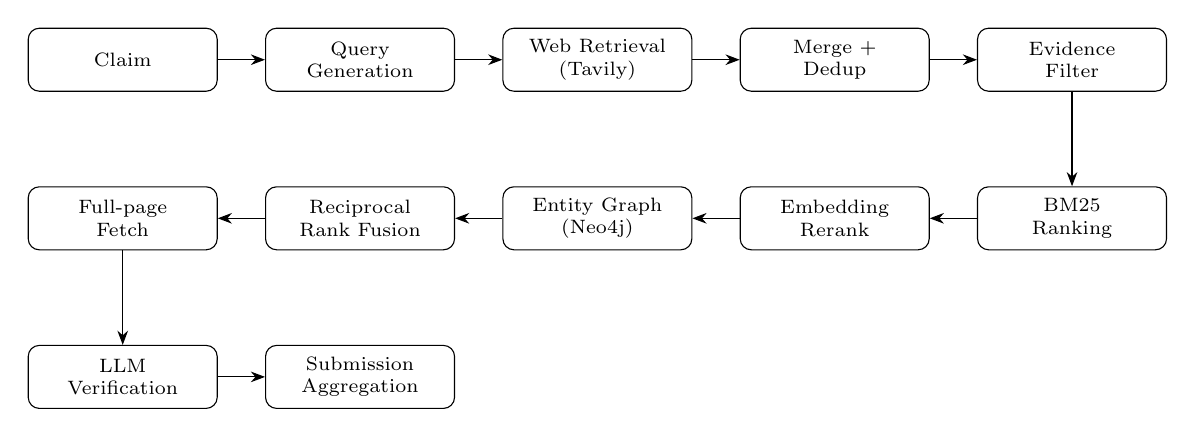
\begin{tikzpicture}[
      node distance=6mm and 6mm,
      box/.style={draw, rounded corners, align=center, minimum height=8mm, minimum width=24mm, font=\scriptsize},
      arr/.style={-{Stealth[length=1.8mm]}}
    ]
    % Row 1
    \node[box] (claim) {Claim};
    \node[box, right=of claim] (qg) {Query\\Generation};
    \node[box, right=of qg] (ret) {Web Retrieval\\(Tavily)};
    \node[box, right=of ret] (merge) {Merge +\\Dedup};
    \node[box, right=of merge] (filt) {Evidence\\Filter};
    % Row 2 (below, reversed direction to save width)
    \node[box, below=12mm of filt] (bm25b) {BM25\\Ranking};
    \node[box, left=of bm25b] (emb) {Embedding\\Rerank};
    \node[box, left=of emb] (ent) {Entity Graph\\(Neo4j)};
    \node[box, left=of ent] (rrf) {Reciprocal\\Rank Fusion};
    \node[box, left=of rrf] (fetch) {Full-page\\Fetch};
    % Row 3
    \node[box, below=12mm of fetch] (llm) {LLM\\Verification};
    \node[box, right=of llm] (sub) {Submission\\Aggregation};

    \draw[arr] (claim) -- (qg);
    \draw[arr] (qg) -- (ret);
    \draw[arr] (ret) -- (merge);
    \draw[arr] (merge) -- (filt);
    \draw[arr] (filt) -- (bm25b);
    \draw[arr] (bm25b) -- (emb);
    \draw[arr] (emb) -- (ent);
    \draw[arr] (ent) -- (rrf);
    \draw[arr] (rrf) -- (fetch);
    \draw[arr] (fetch) -- (llm);
    \draw[arr] (llm) -- (sub);
  \end{tikzpicture}
  \caption{Subtask 2 pipeline. Reads left-to-right, then continues on
    the row below at the rightmost stage of the row above.}
  \label{fig:st2-pipeline}
\end{figure}

\subsection{Query Generation}

Because regional-language news sources are often indexed only in their
own language, we generate \textbf{two} search queries per claim -- one
in the claim's original language, one in English -- rather than relying
on English-only search. Query generation is fully deterministic (no LLM
call): entities are extracted with the same NER pipeline used for the
knowledge-graph stage
(\texttt{Davlan/xlm-roberta-base-ner-hrl} \cite{davlan-xlmr-ner-hrl}),
stopwords are stripped using the \texttt{stopwordsiso} multilingual
stopword lists (unioned across English, Hindi, and Bengali for
code-mixed claims), and a short query is assembled from, in priority
order, (1) exact numeric tokens found verbatim in the claim text (case
counts, percentages, dates), (2) extracted entities kept as intact
multi-word spans, and (3) remaining non-stopword keywords in order of
appearance, capped at eight words. The numeric-token priority was added
after diagnosing a recurring development-set failure pattern: claims
stating a specific statistic were frequently retrieved against a
\emph{different} day's report on the same running story, because the
exact figure was being crowded out of the word budget by generic,
topically-recurring keywords. English translation (used both for the
English query and for downstream embedding reranking) is produced via
\texttt{deep-translator}'s free Google Translate wrapper, with a
raw-text fallback on any translation failure.

\subsection{Web Retrieval and Filtering}

We retrieve results for both queries via the Tavily Search API
\cite{tavily}, scoped to its \texttt{topic="news"} mode (falling back
automatically to unscoped search on any error), merge and deduplicate
the two result sets by URL, and apply a conservative evidence-filtering
pass that removes clear non-article noise -- cookie/terms-of-service/
login pages (detected by URL pattern and exact-title match) and thin,
near-content-free social-media links -- while never removing an item
that would leave the pool empty. This filtering stage was added after
observing that such pages could still score competitively on keyword
overlap alone and occupy a top-3 verification slot without contributing
genuine evidentiary content.

\subsection{BM25 and Embedding Reranking}

The merged, filtered pool is scored twice: once with BM25 (Okapi
variant \cite{robertson2009probabilistic}, corpus-level IDF weighting,
scored against the combined native + English query string, so a single
ranking pass covers evidence in either language), and once with cosine
similarity between the claim's English translation and each evidence
item's title+snippet text, embedded with
\texttt{intfloat/multilingual-e5-base} \cite{wang2024multilingual}
(falling back to \texttt{BAAI/bge-base-en-v1.5} if the preferred model
cannot be loaded), using the \texttt{sentence-transformers} library
\cite{reimers2019sentencebert}. Both stages append their raw score,
min--max-normalized score, and rank to every evidence item, without
modifying or removing any existing field -- every pipeline stage is
additive in this sense, which is what allows Reciprocal Rank Fusion
(Section~\ref{sec:st2-rrf}) to simply read off whichever rank fields it
needs.

\subsection{Entity Graph Ranking}

As in Subtask 1, we build a Neo4j graph -- here with
\texttt{Claim \{id, text, lang, created\_at\}},
\texttt{Evidence \{url, title, snippet, retrieved\_at\}}, and
\texttt{Entity \{normalized\_text, original\_text, qid?\}} nodes,
connected by \texttt{MENTIONS} edges and a
\texttt{MATCHES \{overlap\_raw, overlap\_norm, entity\_rank\}} edge from
each evidence item to the claim it was ranked against. Because the
shared task's open-domain setting has no fixed evidence pool to
pre-link, this graph is \textbf{surface-form-only by default} (entities
are matched by a normalized string comparison, with a
suffix-stripping and substring-containment fallback for Bengali/Hindi
inflected forms), avoiding a per-claim SPARQL dependency on the
retrieval-critical path. We layer an \textbf{optional} Wikidata QID
cross-lingual linking signal on top: for each claim and evidence
entity, we attempt a live Wikidata lookup (rate-limited, disk-cached,
with a circuit breaker that disables further live lookups for the
remainder of a run after a single HTTP 429) and compute a parallel
QID-overlap count. An evidence item's effective overlap score is the
maximum of its surface-form overlap and its QID overlap -- this can
only ever raise a candidate's score relative to surface-form-only
behavior, never lower it, and gracefully degrades to pure surface-form
matching if Wikidata is unreachable or rate-limited. This is what lets
the system recognize, for example, that an English claim mentioning
``Bamangachi'' and its Bengali-script evidence counterpart refer to the
same real-world place, which no amount of string normalization alone
can detect across scripts.

Unlike Subtask 1's graph, this graph is designed to \textbf{accumulate
persistently} across an entire batch run (and across runs) -- the same
real-world entity or article is represented by exactly one shared node
regardless of how many different claims retrieve or mention it, since
nodes are keyed by stable values (normalized entity text, evidence URL)
rather than anything claim-specific.

\begin{figure}[h]
  \centering
  \fbox{\parbox{0.85\linewidth}{\centering\vspace{2.2cm}
    \textbf{[FIGURE PLACEHOLDER]}\\[2mm]
    Neo4j Browser screenshot of the Subtask 2 knowledge graph --
    accumulated \texttt{Claim}/\texttt{Evidence}/\texttt{Entity}
    structure across multiple claims, illustrating a cross-claim
    shared-entity/shared-evidence pattern and (if enabled) a QID-linked
    cross-script entity pair.\vspace{2.2cm}}}
  % Once you have the screenshot, delete the \fbox{...} block above and
  % use, e.g.:
  % \includegraphics[width=0.85\linewidth]{figures/subtask2_kg.png}
  \caption{Subtask 2 knowledge graph structure (Neo4j Browser).}
  \label{fig:st2-kg}
\end{figure}

\subsection{Reciprocal Rank Fusion}
\label{sec:st2-rrf}

We combine the three per-item ranks -- \texttt{bm25\_rank},
\texttt{embedding\_rank}, \texttt{entity\_rank} -- with the standard
Reciprocal Rank Fusion formula \cite{cormack2009reciprocal},
\begin{equation}
  \mathrm{RRF}(d) = \sum_{i} \frac{1}{k + r_i(d)},
\end{equation}
with $k = 60$ (the conventional default, also used as Elasticsearch's
built-in RRF default). We fuse ranks rather than raw scores
deliberately: BM25 scores are unbounded and corpus-dependent, embedding
similarity is roughly bounded in $[0, 1]$, and entity overlap is a
small integer count -- averaging or weighting these directly would let
whichever signal happens to have the largest numeric range dominate the
fusion, whereas ranks are scale-free by construction. Missing ranks (an
item absent from one signal) are simply skipped rather than penalized
with an artificial worst-case value.

\subsection{LLM Verification}
\label{sec:st2-verification}

For the top-3 fusion-ranked evidence items, we fetch the full article
text of each source URL (via \texttt{trafilatura}
\cite{barbaresi2021trafilatura}, with a BeautifulSoup
boilerplate-stripping fallback, and a graceful fallback to the item's
own search-result snippet on total fetch failure), and construct a
single grounded verification prompt asking a large language model to
produce a structured JSON record with three fields: a 100--150-word
evidence summary, an exact \texttt{SUPPORTS}/\texttt{REFUTES}
prediction, and a 100--120-word justification. The prompt enforces
several strict constraints, checked both by instruction and by post-hoc
validation of the model's actual output:

\begin{itemize}
  \item \textbf{No outside knowledge.} The model must reason only over
    the supplied evidence text.
  \item \textbf{No hedging.} Because the task has exactly two labels and
    no ``not enough evidence'' option, the prompt explicitly forbids
    common hedging phrases (``insufficient evidence,'' ``cannot
    verify,'' etc.) in either output field; if one slips through
    anyway, the response is discarded and regenerated (up to two
    additional retries).
  \item \textbf{Language-matched output.} The \texttt{Evidence} and
    \texttt{Justification} fields must be written in the claim's own
    language, while the \texttt{Prediction} field is always required
    to remain the exact English string \texttt{SUPPORTS} or
    \texttt{REFUTES}, regardless of the other two fields' language --
    this was itself a fix for an observed failure where a Bengali claim
    originally produced fully English output, because the model was
    never explicitly told to match the input language.
  \item \textbf{Truncation handling.} Responses cut off by the token
    budget (more likely for Bengali/Hindi text, which tokenizes less
    efficiently than English) are detected explicitly via the model's
    finish-reason signal and retried from scratch, rather than patched
    -- we deliberately never attempt to ``complete'' a truncated
    sentence, since that is itself a form of the hallucination this
    stage is designed to avoid.
\end{itemize}

\paragraph{Backend note.}
Our verification stage currently calls a Gemini-family model
\cite{geminiteam2023gemini} (accessed through Google's
\texttt{google-genai} SDK) as its LLM backend. During development, this
stage was temporarily switched to OpenAI's GPT-4o-mini
\cite{openai2024gpt4omini} to work around a Gemini free-tier daily
quota limitation while processing the full 1{,}009-claim test set, and
was subsequently switched back to Gemini once a suitable, sufficiently
available Gemini model tier was identified. We report this
transparently because it affects which specific model produced which
historical result file; the results reported in
Section~\ref{sec:results-st2} were produced with the pipeline's
current, Gemini-based configuration.

\subsection{Standalone MuRIL Classifier (Subtask 2)}

As a lower-cost, offline-capable alternative to LLM-based verification,
we additionally evaluate the \textbf{identical} fine-tuned MuRIL
classifier described in Section~\ref{sec:st1-veracity}, reused as-is
for Subtask 2 without any retraining on Subtask 2 data. For each claim,
we classify the claim text against the title+snippet text of its
single top-1 fusion-ranked evidence item (the same evidence
representation already used by the BM25/embedding/entity-graph stages,
chosen so this classification path never needs to re-fetch full
article text for every candidate). This is a genuinely separate
prediction path from the LLM-based default submission pipeline -- the
two are never merged into a single default output, and we report both
independently in Section~\ref{sec:results-st2}.

\textbf{Post-submission engineering update.} Since the official
submission, \texttt{run\_pipeline.py} has been extended with a
\texttt{-{}-verifier \{muril, gemini\}} flag; \texttt{muril} is now the
default and the actual backend used for our own subsequent testing,
writing the same verification-record schema described below regardless
of which backend produced it. Under this default, \texttt{Prediction}
still comes from the MuRIL classifier described above (no API key
required), while \texttt{Justification} is now a real, evidence-grounded
explanation of that already-decided prediction generated by
GPT-4o-mini (which never reclassifies), falling back to a flat
templated sentence if no OpenAI API key is configured. The Gemini-based
path documented in Section~\ref{sec:st2-verification} remains fully
available via \texttt{-{}-verifier gemini} and is what produced the
officially submitted and reported results in
Section~\ref{sec:results-st2} -- this update changes our team's own
default for subsequent testing, not the historical submission.

\subsection{Submission Aggregation}

Every claim's finished verification record -- regardless of which
\texttt{-{}-verifier} backend produced it -- is aggregated into one
final JSON array, validating that every prediction label is exactly
\texttt{SUPPORTS} or \texttt{REFUTES} before writing. The pipeline is
fully resumable: every stage checks for its own already-written output
file and skips claims already completed, so an interrupted
1{,}009-claim batch run over a rate-limited external API can simply be
restarted rather than redone from scratch, and a single claim's failure
at any stage is logged and skipped rather than aborting the batch.

% ============================================================================
\section{Experimental Setup}
% ============================================================================

Table~\ref{tab:setup} summarizes the components, models, and key
hyperparameters used across both subtasks.

\begin{table}[h]
  \centering
  \caption{Experimental setup summary.}
  \label{tab:setup}
  \small
  \begin{tabular}{@{}p{0.30\linewidth}p{0.32\linewidth}p{0.32\linewidth}@{}}
    \toprule
    Component & Subtask 1 & Subtask 2 \\
    \midrule
    Dense/embedding model & \texttt{multilingual-e5-base} & \texttt{multilingual-e5-base} (fallback: \texttt{bge-base-en-v1.5}) \\
    NER model & \texttt{ai4bharat/IndicNER} & \texttt{Davlan/xlm-roberta-base-ner-hrl} \\
    Graph database & Neo4j 5.26 Community + APOC & Neo4j 5.26 Community + APOC \\
    Lexical ranker & \texttt{rank\_bm25} (Okapi) & \texttt{rank\_bm25} (Okapi) \\
    Web search API & --- (closed pool) & Tavily (\texttt{topic="news"}) \\
    Veracity LLM & GPT-4o-mini & Gemini family \\
    Standalone classifier & MuRIL, fine-tuned & Same checkpoint, reused \\
    Classifier max seq.\ length & 192 tokens & 192 tokens \\
    Classifier precision & \texttt{fp16} & \texttt{fp16} (same checkpoint) \\
    HPO & Optuna, 15 trials & Optuna, 15 trials (same search) \\
    Entity-overlap rerank weight & 0.02 (swept $[0.0, 2.0]$) & N/A (surface-form + optional QID, max-combine) \\
    Evidence pool & 13{,}333 / 28{,}618 (dev/test) & Open web, top-6 per query \\
    RRF constant $k$ & N/A & 60 \\
    Fusion signals & N/A & BM25 rank, embedding rank, entity rank \\
    \bottomrule
  \end{tabular}
\end{table}

All dense/embedding-model encodings are cached to disk to avoid
redundant recomputation across ablations and repeated pipeline runs.
Both pipelines run entity extraction and Neo4j graph writes as
resumable batch stages -- network-facing lookups (Wikidata SPARQL,
\texttt{wbsearchentities}, Wikipedia redirect resolution) are all
disk-cached with an explicit staleness check tied to specific
documented bug fixes, so a corrected pipeline is guaranteed not to
silently keep serving pre-fix cached results.

% ============================================================================
\section{Results}
% ============================================================================

\subsection{Subtask 1}
\label{sec:results-st1}

\begin{table}[h]
  \centering
  \caption{Official test-set results for Subtask 1 (ClaimSense,
    Submission 1). The results sheet reports Subtask 1a (Evidence
    Retrieval) and Subtask 1b (Veracity Prediction) separately, per
    language.}
  \label{tab:st1-official}
  \small
  \begin{tabular}{@{}lrrrrrr@{}}
    \toprule
    & \multicolumn{3}{c}{Subtask 1a -- Retrieval} & \multicolumn{3}{c}{Subtask 1b -- Veracity} \\
    \cmidrule(lr){2-4} \cmidrule(lr){5-7}
    Language & Success@3 & MRR@3 & nDCG@3 & Precision & Recall & Macro-F1 \\
    \midrule
    English     & 79.58 & 49.67 & 57.54 & 78.26 & 78.08 & 78.05 \\
    Hindi       & 88.67 & 51.99 & 61.28 & 88.26 & 86.08 & 85.88 \\
    Bengali     & 67.00 & 38.99 & 46.08 & 84.42 & 83.50 & 82.46 \\
    Code-mixed  & 26.67 & 22.33 & 23.44 & 80.35 & 80.00 & 79.94 \\
    \bottomrule
  \end{tabular}
\end{table}

\begin{table}[h]
  \centering
  \caption{Development-set retrieval ablation (Success@3 / nDCG@3),
    our own internal validation used to select the final production
    configuration.}
  \label{tab:st1-ablation}
  \small
  \begin{tabular}{@{}lrlllll@{}}
    \toprule
    Method & $n$ & Hindi & Bengali & English & Code-mixed & Overall \\
    \midrule
    BM25 & 1{,}134 & 0.889/0.607 & 0.670/0.488 & 0.796/0.629 & 0.662/0.470 & 0.768/0.563 \\
    Dense (full-pool) & 1{,}134 & 0.875/0.584 & 0.682/0.488 & 0.869/0.623 & 0.773/0.512 & 0.818/0.566 \\
    Dense (partitioned) & 1{,}134 & 0.875/0.575 & 0.687/0.490 & 0.874/0.626 & 0.773/0.512 & 0.821/0.565 \\
    Dense-only & 5{,}670 & 0.882/0.567 & 0.739/0.539 & 0.882/0.634 & 0.767/0.505 & 0.831/0.571 \\
    \textbf{KG-boosted} & 5{,}670 & 0.883/0.568 & 0.756/0.547 & 0.889/0.635 & 0.780/0.512 & \textbf{0.8395/0.5748} \\
    \bottomrule
  \end{tabular}
\end{table}

\begin{table}[h]
  \centering
  \caption{Entity-overlap weight sweep (KG-boosted reranking, all
    5{,}670 train+dev claims, one Neo4j pass reused across every weight
    tried).}
  \label{tab:sweep}
  \small
  \begin{tabular}{@{}rrrl@{}}
    \toprule
    Weight & Success@3 & nDCG@3 & \\
    \midrule
    0.00 & 0.8312 & 0.5713 & (= dense-only; sanity check) \\
    0.01 & 0.8376 & 0.5746 & beats dense-only \\
    0.015 & 0.8383 & 0.5749 & beats dense-only \\
    \textbf{0.02} & \textbf{0.8395} & \textbf{0.5748} & \textbf{best -- beats dense-only on both} \\
    0.025 & 0.8377 & 0.5742 & beats dense-only \\
    0.03 & 0.8379 & 0.5736 & beats dense-only \\
    0.04 & 0.8388 & 0.5738 & beats dense-only \\
    0.05 & 0.8381 & 0.5733 & beats dense-only \\
    0.10 & 0.8231 & 0.5664 & below dense-only again \\
    0.20 & 0.8035 & 0.5542 & far below \\
    \bottomrule
  \end{tabular}
\end{table}

\begin{table}[h]
  \centering
  \caption{Development-set veracity prediction, both scored on the same
    KG-boosted top-3 evidence.}
  \label{tab:st1-veracity}
  \small
  \begin{tabular}{@{}lrrr@{}}
    \toprule
    Model & $n$ & Accuracy & Macro-F1 \\
    \midrule
    MuRIL classifier & 1{,}134 (dev) & 0.8660 & 0.8480 \\
    GPT-4o-mini & 1{,}134 (dev) & \textbf{0.9198} & \textbf{0.9075} \\
    GPT-4o-mini & 5{,}670 (train+dev) & --- & 0.9236 \\
    \bottomrule
  \end{tabular}
\end{table}

\paragraph{Discussion.}
KG-boosted reranking beats dense-retrieval-only on both metrics at
every entity-overlap weight tried in $[0.01, 0.05]$ -- a real, robust
improving region, not a single lucky configuration. GPT-4o-mini
outperforms our fine-tuned MuRIL classifier on veracity prediction by a
wide margin (macro-F1 0.9075 vs.\ 0.8480 on the same 1{,}134-claim dev
set and same evidence). Bengali and code-mixed are consistently the
weakest retrieval buckets across every method tested, a known weak
point of general-purpose multilingual embedding models and, for
code-mixed text specifically, of script-based language detection
generally.

\subsection{Subtask 2}
\label{sec:results-st2}

\begin{table}[h]
  \centering
  \caption{Official test-set results for Subtask 2 (ClaimSense,
    Submission 1) -- the Gemini-based LLM verification path
    (Section~\ref{sec:st2-verification}); the standalone MuRIL
    classifier was not submitted and has no official row of its own.}
  \label{tab:st2-official}
  \small
  \begin{tabular}{@{}lrrr@{}}
    \toprule
    Language & Precision & Recall & Macro-F1 \\
    \midrule
    English & 77.02 & 76.93 & 76.91 \\
    Hindi & 68.86 & 68.76 & 68.97 \\
    Bengali & 62.88 & 63.09 & 62.92 \\
    Code-mixed & 54.06 & 57.00 & 36.51 \\
    \midrule
    \textbf{Unweighted average} & \textbf{65.71} & \textbf{66.45} & \textbf{61.33} \\
    \bottomrule
  \end{tabular}
\end{table}

The unweighted per-language average is our own computation from the
four rows above (the results sheet does not publish a separate pooled
``Overall'' figure for this system); we report it only as a convenient
single-number summary, not as an official metric in its own right. The
most striking result here is \textbf{code-mixed Macro-F1 collapsing to
36.51} -- far below its own Precision/Recall (54.06/57.00) and far
below every other language's Macro-F1 -- indicating a highly imbalanced
or degenerate prediction pattern specifically on code-mixed claims at
official test time, a more severe version of the code-mixed weakness we
also observe throughout Subtask 1's retrieval results
(Section~\ref{sec:results-st1}) and discuss further in
Section~\ref{sec:discussion}.

\begin{table}[h]
  \centering
  \caption{Development-set veracity prediction (631 claims, gold
    labels), our own internal comparison between the submitted LLM path
    and the non-submitted, reused MuRIL classifier -- one row per
    claim, comparing each system's actual final \texttt{Prediction}
    against gold \texttt{Label}. Distinct from Table~\ref{tab:st2-official}'s
    official per-language test-set numbers.}
  \label{tab:st2-dev}
  \small
  \begin{tabular}{@{}lrrrr@{}}
    \toprule
    System & Accuracy & Macro-F1 & F1 (S) & F1 (R) \\
    \midrule
    \textbf{LLM verification (Gemini)} -- submitted & \textbf{0.8082} & \textbf{0.8039} & \textbf{0.8331} & \textbf{0.7747} \\
    MuRIL classifier -- not submitted & 0.7005 & 0.6820 & 0.7586 & 0.6054 \\
    \bottomrule
  \end{tabular}
\end{table}

\paragraph{A methodological note we report transparently.}
An earlier internal evaluation of the MuRIL classifier's
development-set performance reported a substantially lower accuracy
(0.5563), because it scored every individual (claim, evidence) pair the
classifier was run against (1{,}891 rows: up to three candidate
evidence items per claim), rather than the single final prediction
actually used per claim, as the LLM path's own metric does. We
identified and corrected this inconsistency before finalizing the
comparison above; the corrected number (0.7005 accuracy) is the one we
report as authoritative, computed on exactly the same 631-claim,
one-row-per-claim basis as the LLM path.

We additionally note one remaining asymmetry between the two systems
compared in Table~\ref{tab:st2-dev}: the LLM verification path reads
the \emph{full fetched article text} of its top-3 evidence sources,
while the MuRIL classifier -- to avoid re-fetching every candidate URL
a second time -- is scored against only the top-ranked item's
search-result title and snippet. Part of the accuracy gap in
Table~\ref{tab:st2-dev} may therefore reflect this input-quality
difference rather than model capability alone; we flag this as a
controlled follow-up experiment for future work
(Section~\ref{sec:future-work}). Note also that
Table~\ref{tab:st2-official} (official test set) and
Table~\ref{tab:st2-dev} (our own dev split) are not directly comparable
to each other -- different claims, and Table~\ref{tab:st2-official} is
broken down per language while Table~\ref{tab:st2-dev} is pooled -- so
the gap between them should not be read as a single clean number; the
code-mixed collapse in Table~\ref{tab:st2-official} is doing most of
that work on its own, as the per-language breakdown shows.

% ============================================================================
\section{Error Analysis and Discussion}
\label{sec:discussion}
% ============================================================================

\paragraph{Code-mixed veracity prediction collapses on the official
Subtask 2 test set.}
Table~\ref{tab:st2-official}'s code-mixed row shows Precision 54.06 and
Recall 57.00 -- already the weakest of the four languages, but not
dramatically so -- alongside a Macro-F1 of only 36.51, a much larger
drop than Precision/Recall alone would suggest. A Macro-F1 this far
below both its own Precision/Recall and every other language's
Macro-F1 is a signature of a degenerate or heavily skewed prediction
pattern (for instance, the system defaulting toward one label far more
often than the true code-mixed label distribution warrants, which
depresses the \emph{minority} class's F1 sharply even while
Precision/Recall averaged another way look only moderately weak). We
had no comparably sized, per-language-labeled internal held-out set for
Subtask 2's official test distribution specifically to catch this
before submission -- our own development-set numbers
(Table~\ref{tab:st2-dev}) are pooled across languages, not broken out
by language, which is precisely the kind of blind spot that let this
pattern go undetected internally.

\paragraph{Bengali and code-mixed retrieval are the hardest conditions
across both subtasks.}
In Subtask 1, code-mixed Success@3 lags every other language bucket by
a wide margin regardless of retrieval method (e.g., 0.780 KG-boosted
vs.\ 0.889 for English); Bengali is consistently second-weakest. We
attribute this to two compounding factors: general-purpose multilingual
sentence embeddings are typically trained on far less Bengali data than
English or Hindi, and code-mixed claims by definition straddle two or
more scripts within a single sentence, which both weakens
single-language keyword overlap for BM25 and can confuse script-based
language routing.

\paragraph{Entity-overlap reranking is a real but narrow improvement.}
The KG-boosted reranking stage's gain over dense-retrieval-only is real
and validated by a full weight sweep (Table~\ref{tab:sweep}), but it is
a modest absolute improvement (Success@3 $+0.0083$ at the best weight)
-- appropriate for a signal designed to \emph{disambiguate near-ties}
in the dense top-10, not to override dense retrieval's primary ranking.

\paragraph{Cluster-density penalties do not help at production scale,}
despite being a reasonable hypothesis. Our controlled experiment
(Section~\ref{sec:st1-kg}) showed this degrades monotonically as the
penalty weight increases, because the clustering threshold that worked
on a small, single-story validation set collapsed into one dominant
cluster per language at full corpus scale. We view this as a useful
negative result: a disambiguation signal that only works at a smaller
scale than the deployed system is not safe to deploy without
re-validating the clustering threshold at the actual production scale.

\paragraph{LLM-based veracity prediction consistently and substantially
outperforms our fine-tuned classifier,} on both subtasks (Subtask 1:
macro-F1 0.9075 vs.\ 0.8480; Subtask 2: macro-F1 0.8039 vs.\ 0.6820, dev
set). We consider two likely, non-exclusive explanations: (i)
GPT-4o-mini and Gemini are general-purpose models with substantially
larger pretraining exposure to multilingual and code-mixed text than a
180M-parameter fine-tuned MuRIL classifier, and (ii) the LLM paths
reason over richer context (a full evidence passage or full fetched
article, versus the classifier's shorter,
\texttt{max\_length=192}-token-truncated input) -- a difference we
explicitly flag as a confound worth isolating in future work rather
than treating this comparison as a clean measure of ``LLM vs.\
fine-tuned model'' capability alone.

\paragraph{The verification stage's strict anti-hedging design is a
deliberate response to the task's binary-only label space.} Because
FIRE 2026 provides no ``insufficient evidence'' label, a system that
defaults to a mechanical ``evidence is thin $\rightarrow$ REFUTES''
rule would systematically misclassify genuinely under-evidenced
SUPPORTS claims. Our prompt explicitly bans this shortcut and checks
for it post-hoc; we consider this a necessary design choice given the
task's label space, not an optional refinement.

% ============================================================================
\section{Limitations and Future Work}
\label{sec:future-work}
% ============================================================================

\begin{itemize}
  \item \textbf{Wikidata linking coverage.} Our entity-linking cascade
    is grounded entirely in Wikidata, which has known coverage gaps for
    minor regional entities, informal organization names, and very
    recent events -- a mention with no Wikidata presence at all cannot
    be resolved by any stage of our cascade, LLM fallback included.
  \item \textbf{Evidence representation parity for the Subtask 2
    classifier comparison.} As noted in Section~\ref{sec:results-st2},
    the MuRIL classifier and the LLM verification path are not
    currently evaluated on identical evidence text. A controlled
    follow-up giving the classifier the same full-article text as the
    LLM path would isolate model capability from input-quality as the
    source of their performance gap.
  \item \textbf{Event-clustering disambiguation} remains an open
    problem at production scale; our experiment shows the
    \emph{current} DBSCAN-based approach does not help, not that no
    clustering-based signal could help with a better-calibrated
    threshold or a different clustering algorithm.
  \item \textbf{Live web retrieval instability (Subtask 2).} Web search
    results for a given query can change over time, meaning Subtask 2
    evaluation is not perfectly reproducible run-to-run in the way
    Subtask 1's fixed-pool evaluation is -- a structural property of
    the open-domain setting rather than a defect in our system.
  \item \textbf{Code-mixed-specific modeling.} Both subtasks currently
    treat code-mixed text largely as ``apply every relevant language's
    tooling and union the results'' rather than using any
    code-mixing-aware model or normalization step; given that
    code-mixed claims are the weakest bucket across every method we
    tested, a dedicated code-mixed normalization or embedding
    fine-tuning pass is a promising direction.
  \item \textbf{Per-language development monitoring, not just a single
    pooled dev metric.} The official Subtask 2 code-mixed Macro-F1
    collapse (Section~\ref{sec:discussion}) was not visible in our own
    pooled, all-languages development metric before submission.
    Tracking Precision/Recall/Macro-F1 separately per language during
    development -- mirroring exactly how the shared task itself reports
    results -- would very likely have surfaced this specific failure
    mode in time to address it before the official run.
\end{itemize}

% ============================================================================
\section{Conclusion}
% ============================================================================

We presented ClaimSense's system for both subtasks of
IndicClaimVer@FIRE 2026. Our Subtask 1 system combines dense
multilingual retrieval with an IDF-weighted, Wikidata-grounded
knowledge-graph reranking stage, validated by a full hyperparameter
sweep to robustly improve over dense retrieval alone, paired with
either an LLM-based or a fine-tuned-classifier veracity predictor; on
the official test set it reaches a veracity Macro-F1 of 78.05--85.88
across English, Hindi, and Bengali, and 79.94 on code-mixed. Our
Subtask 2 system generates bilingual search queries deterministically,
retrieves and ranks open-web evidence through a three-signal
Reciprocal-Rank-Fusion pipeline, and produces grounded,
anti-hallucination-constrained veracity verdicts via an LLM, with a
reused standalone classifier evaluated internally as a lower-cost
alternative (not submitted); on the official test set it reaches a
veracity Macro-F1 of 62.92--76.91 across English, Hindi, and Bengali,
but collapses to 36.51 on code-mixed -- the single most actionable
finding of this paper, and one we did not detect internally before
submission due to using only a pooled, not per-language, development
metric. Across both subtasks, LLM-based veracity prediction
meaningfully outperforms our fine-tuned MuRIL classifier on our own
internal comparison, and Bengali/code-mixed text remains the consistent
weak point for both retrieval quality and, on the official Subtask 2
test set specifically, veracity prediction itself.

% ============================================================================
\begin{acknowledgments}
% ============================================================================
We thank the IndicClaimVer@FIRE 2026 organizers for creating and
running this shared task, and for providing the IndicClaimBuster
dataset underlying both subtasks.
\end{acknowledgments}

% ============================================================================
\section*{Declaration on Generative AI}
% ============================================================================
% CEUR-WS has required this section since January 2025. Edit to reflect
% actual usage before submission -- the text below is a starting draft,
% not a verified final statement.
During the preparation of this work, the authors used [an AI coding/
writing assistant -- name and version placeholder] to assist with code
review, documentation, and drafting portions of this manuscript. All
reported experimental results, system designs, and conclusions were
reviewed and verified by the authors, who take full responsibility for
the content of this publication.

% ============================================================================
\bibliography{references}
% ============================================================================

\end{document}
